% CoLLAs 2026 submission — using official style file
%
% ── OpenReview submission metadata (not rendered) ──────────────────
% Title: Basin Fragmentation Predicts Regularization Benefit in Continual
%        Learning Under Dataset-Dependent Regimes
% Author OpenReview ID: ~Joshua_R_Gutierrez2
% Keywords: continual learning; catastrophic forgetting; persistent homology;
%           loss landscape geometry; elastic weight consolidation
% TL;DR: Persistent homology of loss landscape cross-sections predicts the
%        magnitude of EWC benefit in continual learning, with dataset-dependent
%        regimes and method specificity (no signal for SI).
% ───────────────────────────────────────────────────────────────────
\documentclass{article}
\usepackage{collas2026_conference,times}

% Additional packages
\usepackage{amsmath,amssymb}
\usepackage{graphicx}
\usepackage{booktabs}
\usepackage{hyperref}
\hypersetup{hidelinks}
\usepackage{xcolor}
\usepackage[expansion=false]{microtype}
\usepackage{multirow}
\usepackage{enumitem}

%\collasfinalcopy % Uncomment for camera-ready version, but NOT for submission.

\title{Basin Fragmentation Predicts Regularization Benefit in Continual Learning\\Under Dataset-Dependent Regimes}

\author{Antiquus S.~Hippocampus \\
Department of Computer Science\\
Random University\\
\texttt{hippo@cs.random.edu}}

\newcommand{\fix}{\marginpar{FIX}}
\newcommand{\new}{\marginpar{NEW}}

% ════════════════════════════════════════════════════════════════
\begin{document}

\maketitle

% ════════════════════════════════════════
\begin{abstract}
We introduce a geometric perspective on mitigation sensitivity in continual learning. Using persistent homology to extract topological features from loss landscape cross-sections, we show that landscape topology provides predictive signal for regularization benefit in specific regimes, with identifiable boundary conditions. Across 19 architectures and 3 datasets (57 configurations, 0.3M--44.7M parameters trained from scratch at 32$\times$32), $H_0$ (connected components) is predictive of EWC benefit after controlling for model capacity and standard landscape statistics (sharpness, Fisher trace, loss barrier, weight norm): on RESISC-45, topology explains more variance than model size ($R^2 = 0.645$ vs.\ $0.242$, $p < 0.001$) and retains significance after controlling for every baseline ($p < 0.001$), with partial replication on CIFAR-100 and a null on CUB-200; pooled across datasets ($n = 57$), $H_0$ retains significance ($p = 0.012$). Preliminary scale validation on ImageNet-100 (8 pretrained architectures, 20M--304M parameters at 224$\times$224) suggests that $H_1$ (loops), not $H_0$, may carry the topological signal at larger scale ($\rho = 0.93$, $p = 0.0007$), though $n = 8$ and a different training regime limit the strength of this observation. A key discriminator: testing synaptic intelligence (SI) as a second curvature-aware method yields zero topology moderation ($p = 1.000$), sharpening the hypothesis to EWC-specific rather than general regularization effects. We propose the \emph{basin fragmentation hypothesis}, provide explicit falsification targets, and report which have been addressed.
\end{abstract}

% ════════════════════════════════════════
\section{Introduction}
\label{sec:intro}

Catastrophic forgetting, the abrupt loss of previously learned knowledge during sequential training, remains a central obstacle in continual learning \citep{mccloskey1989catastrophic, french1999catastrophic}. Mitigation strategies including elastic weight consolidation \citep[EWC;][]{kirkpatrick2017overcoming}, synaptic intelligence \citep{zenke2017continual}, and replay-based methods \citep{rebuffi2017icarl} differ fundamentally in mechanism, yet practitioners select among them by trial and error. A diagnostic that predicts which method will help, and by how much, before committing to sequential training would change how continual learning systems are deployed.

Recent work has established that loss landscape geometry encodes meaningful information about generalization \citep{li2018visualizing, keskar2017on} and mode connectivity \citep{garipov2018loss}. Separately, persistent homology has emerged as a principled framework for characterizing multi-scale structure in high-dimensional data \citep{carlsson2009topology}. We bridge these two lines by asking: \textbf{does the topological structure of a model's loss landscape predict how much a given mitigation method will help?}

We answer affirmatively for EWC, with important caveats. Our contributions:

\begin{enumerate}[nosep,leftmargin=*]
    \item \textbf{A geometric lens on mitigation sensitivity.} We show that persistent homology from loss landscape topology provides predictive signal for the magnitude of EWC benefit, under specific dataset conditions. This shifts the framing from ``does topology correlate with forgetting?'' to ``does topology indicate which models benefit from which interventions?''

    \item \textbf{Capacity-controlled evidence and baseline comparison.} Per-dataset controlled regressions establish that $H_0$ is not merely a proxy for model size or standard landscape statistics. $H_0$ retains significance after controlling for parameter count ($p = 0.012$ pooled), and partial correlation analysis shows $H_0$ captures predictive signal beyond Hessian trace (sharpness), max eigenvalue, Fisher trace, loss barrier, and L2 weight norm, while most baselines do not retain significance after controlling for $H_0$.

    \item \textbf{Preliminary scale validation.} On ImageNet-100 (8 pretrained architectures, 20M--304M parameters), $H_1$ (loops) shows a strong correlation with retention ($\rho = 0.93$, $p = 0.0007$) where $H_0$ does not, suggesting that the informative topological dimension may shift with scale. This observation requires replication.

    \item \textbf{Method specificity as a key discriminator.} SI shows zero topology moderation ($p = 1.000$), sharpening the hypothesis from ``topology predicts regularization benefit'' to ``topology predicts EWC-specific benefit.'' This narrows the mechanism and provides preliminary evidence against a trivially general interpretation.

    \item \textbf{Cross-architecture, cross-dataset evaluation.} 27 architectures spanning CNNs, Vision Transformers, and MLP-based designs across 4 datasets (65 total configurations). Open-source release of all code and results.\footnote{URL withheld for review.}
\end{enumerate}

% ════════════════════════════════════════
\section{Related Work}
\label{sec:related}

\textbf{Continual learning.} Forgetting mitigation methods fall into regularization-based \citep{kirkpatrick2017overcoming, zenke2017continual}, replay-based \citep{rebuffi2017icarl, shin2017continual}, and architecture-based \citep{rusu2016progressive, mallya2018packnet} categories. EWC \citep{kirkpatrick2017overcoming} penalizes changes to parameters deemed important by the Fisher information matrix. Our work is orthogonal to method development: we ask whether pre-training landscape properties predict how much a given method helps.

\textbf{Loss landscape analysis.} \citet{li2018visualizing} introduced filter-normalized random directions for cross-architecture landscape visualization. \citet{keskar2017on} linked sharpness to generalization. \citet{garipov2018loss} demonstrated mode connectivity. These studies are descriptive: they characterize landscape geometry but do not connect it to actionable continual learning decisions. We move from visualization to prediction.

\textbf{TDA in deep learning.} Persistent homology has been applied to decision boundaries \citep{ramamurthy2019topological}, weight-space topology \citep{rieck2019neural}, and activation patterns \citep{naitzat2020topology}. Our work differs in applying persistent homology to loss landscape \emph{surfaces} and relating the extracted features to mitigation-specific outcomes in continual learning.

% ════════════════════════════════════════
\section{Methodology}
\label{sec:method}

\subsection{Experimental Design}

\textbf{Small-scale study (from scratch, 32$\times$32).} We evaluate 19 architectures spanning CNNs, Vision Transformers, and MLP-based designs (Table~\ref{tab:architectures}), including a WRN-28-$k$ width ladder ($k \in \{1,2,4,6,8,10\}$) that isolates capacity effects within a single architecture family. Parameter counts range from 0.3M (ViT-Tiny) to 44.7M (ResNet-18 Wide). All models are trained from scratch on three datasets selected for domain diversity: CIFAR-100 (natural images, 50/50 class split), CUB-200-2011 \citep{wah2011caltech} (fine-grained birds, 100/100 split), and NWPU-RESISC45 \citep{cheng2017remote} (satellite scenes, 23/22 split). All images are resized to $32 \times 32$ for cross-architecture consistency.

\textbf{Scale validation (pretrained, 224$\times$224).} To test whether the topological signal extends beyond small-scale models, we evaluate 8 additional architectures on ImageNet-100 \citep{deng2009imagenet} (a 100-class subset, 50/50 split) at $224 \times 224$ resolution using pretrained ImageNet-1K weights fine-tuned with AdamW (lr $= 10^{-4}$, cosine schedule, 30 epochs). Parameter counts range from 20M (DenseNet-201) to 304M (ViT-L/16). This constitutes a different experimental regime: pretrained fine-tuning rather than from-scratch training, with models up to $7\times$ larger than the small-scale study.

\begin{table}[t]
\centering
\caption{Architectures evaluated. \textbf{Top:} 19 small-scale architectures trained from scratch at 32$\times$32 on CIFAR-100, CUB-200, and RESISC-45 (57 configs). \textbf{Bottom:} 8 scale-validation architectures fine-tuned from pretrained weights at 224$\times$224 on ImageNet-100 (8 configs).}
\label{tab:architectures}
\small
\begin{tabular}{@{}lrl@{}}
\toprule
Architecture & Params & Type \\
\midrule
\multicolumn{3}{@{}l}{\textit{Small-scale (from scratch, 32$\times$32)}} \\
ViT-Tiny         & 0.3M  & Transformer \\
WRN-28-1         & 0.4M  & WRN ladder \\
MobileNet-V3-S   & 1.1M  & CNN \\
ShuffleNet-V2    & 1.3M  & CNN \\
WRN-28-2         & 1.5M  & WRN ladder \\
ViT-Small        & 2.2M  & Transformer \\
MLP-Mixer        & 2.3M  & MLP \\
RegNet-Y-400MF   & 4.0M  & CNN \\
EfficientNet-B0  & 4.1M  & CNN \\
WRN-28-4         & 5.9M  & WRN ladder \\
DenseNet-121     & 7.1M  & CNN \\
ResNet-18        & 11.2M & CNN \\
WRN-28-6         & 13.2M & WRN ladder \\
VGG-16-BN        & 14.8M & CNN \\
WRN-28-8         & 23.4M & WRN ladder \\
ResNet-50        & 23.7M & CNN \\
ConvNeXt-Tiny    & 27.9M & Modern CNN \\
WRN-28-10        & 36.5M & WRN ladder \\
ResNet-18 Wide   & 44.7M & CNN \\
\midrule
\multicolumn{3}{@{}l}{\textit{Scale validation (pretrained, 224$\times$224)}} \\
DenseNet-201     & 20M   & CNN \\
EfficientNet-B5  & 30M   & CNN \\
ResNet-101       & 44M   & CNN \\
ConvNeXt-Small   & 50M   & Modern CNN \\
ViT-B/16         & 86M   & Transformer \\
ConvNeXt-Base    & 89M   & Modern CNN \\
ConvNeXt-Large   & 198M  & Modern CNN \\
ViT-L/16         & 304M  & Transformer \\
\bottomrule
\end{tabular}
\end{table}

\subsection{Loss Landscape Topology}
\label{sec:topology}

For each converged model $\boldsymbol{\theta}^*$, we compute persistent homology on 2D cross-sections of the loss landscape. For each of 5 independent random seeds, two random directions $\mathbf{d}_1, \mathbf{d}_2$ in parameter space are generated with filter normalization \citep{li2018visualizing}, and loss is evaluated on a $50 \times 50$ grid over $[-1,1]^2$:
\begin{equation}
    \mathcal{L}(\alpha, \beta) = \mathcal{L}\!\left(\boldsymbol{\theta}^* + \alpha\,\mathbf{d}_1 + \beta\,\mathbf{d}_2\right).
\end{equation}

We compute $H_0$ (connected components) and $H_1$ (loops) via Ripser \citep{bauer2021ripser} using lower-star filtration on the 8-adjacency graph, with GUDHI cubical persistence as a validation baseline ($H_1$ agreement $\rho = 1.0$ on all datasets). Five slices per architecture reduces sampling variance compared to single-slice designs.

\subsection{Forgetting and Mitigation Measurement}

From each Task A checkpoint, we train on Task B under three conditions:
\begin{itemize}[nosep,leftmargin=*]
    \item \textbf{Naive:} SGD with momentum, fixed LR.
    \item \textbf{EWC:} Naive training plus elastic weight consolidation ($\lambda = 1000$) \citep{kirkpatrick2017overcoming}.
    \item \textbf{SI:} Naive training plus synaptic intelligence ($c = 1.0$) \citep{zenke2017continual}. Tested on ImageNet-100 to evaluate method specificity.
\end{itemize}

Task A accuracy is evaluated at steps $\{10, 25, 50, 100, 250, 500, 1000, 5000\}$. Retention is $\text{ret}@k = \text{acc}_A(k) / \text{acc}_A(0)$. EWC benefit is the absolute improvement:
\begin{equation}
    \text{EWC\_benefit} = \text{AURC}_{\text{EWC}} - \text{AURC}_{\text{naive}}
\end{equation}
where AURC is the area under the retention curve (trapezoidal, steps 0--500).

\subsection{Statistical Analysis}

\textbf{Per-dataset correlations.} Spearman rank correlations between $H_0$, $H_1$, parameter count, and EWC benefit, with Bonferroni correction.

\textbf{Controlled regression (key test).} Per-dataset OLS:
\begin{equation}
    \text{EWC\_benefit} = \beta_0 + \beta_1 \log(\text{params}) + \beta_2 H_0 + \epsilon
    \label{eq:controlled}
\end{equation}
If $\beta_2$ is significant, $H_0$ is not merely a capacity proxy. We additionally test a model including architectural depth (weight-bearing layer count) as a third predictor.

\textbf{Partial correlation.} Residualize both $H_0$ and EWC benefit on $\log(\text{params})$, then compute Spearman $\rho$ on the residuals. This provides a nonparametric complement to the OLS test.

\textbf{Per-dataset LOAO prediction.} For each held-out architecture, fit a Ridge model on the remaining $n - 1$ architectures and predict the held-out retention. Nested alpha selection via inner leave-one-out. We compare three feature sets: params-only, topology-only ($H_0$, $H_1$), and params + topology. A permutation test (1000 shuffles of topology columns) determines whether topology improves prediction beyond params.

\textbf{Pooled interaction model.} All observations pooled with dataset indicators:
\begin{align}
    \text{M0:}&\quad Y = \beta_0 + \beta_1 \hat{p} + \beta_2 D_C + \beta_3 D_R + \beta_4 \hat{p}D_C + \beta_5 \hat{p}D_R + \epsilon \\
    \text{M1:}&\quad Y = \text{M0} + \gamma_1 \tilde{H}_0 + \gamma_2 \tilde{H}_0 D_C + \gamma_3 \tilde{H}_0 D_R + \epsilon
\end{align}
where $\hat{p} = \log(\text{params})$ globally standardized, $\tilde{H}_0$ is $H_0$ z-scored within each dataset, and $D_C$, $D_R$ are dataset indicators. Significance via permutation test (1000 shuffles) and 95\% clustered bootstrap CIs (5000 iterations, resampling architecture blocks).

% ════════════════════════════════════════
\section{Results}
\label{sec:results}

\subsection{H0 Predicts EWC Benefit (Small Scale)}

Table~\ref{tab:ewc_corr} and Figure~\ref{fig:h0_ewc_scatter} present the core finding. $H_0$ persistence correlates with EWC benefit on 2 of 3 datasets: CIFAR-100 ($\rho = 0.76$, $p = 0.0002$) and RESISC-45 ($\rho = 0.86$, $p = 2.4 \times 10^{-6}$), with CUB-200 showing a null ($\rho = 0.31$, $p = 0.19$). The CIFAR-100 and RESISC-45 correlations survive Bonferroni correction across 3 datasets and are corroborated by Kendall $\tau$ ($0.57$ and $0.67$).

\begin{figure}[t]
\centering
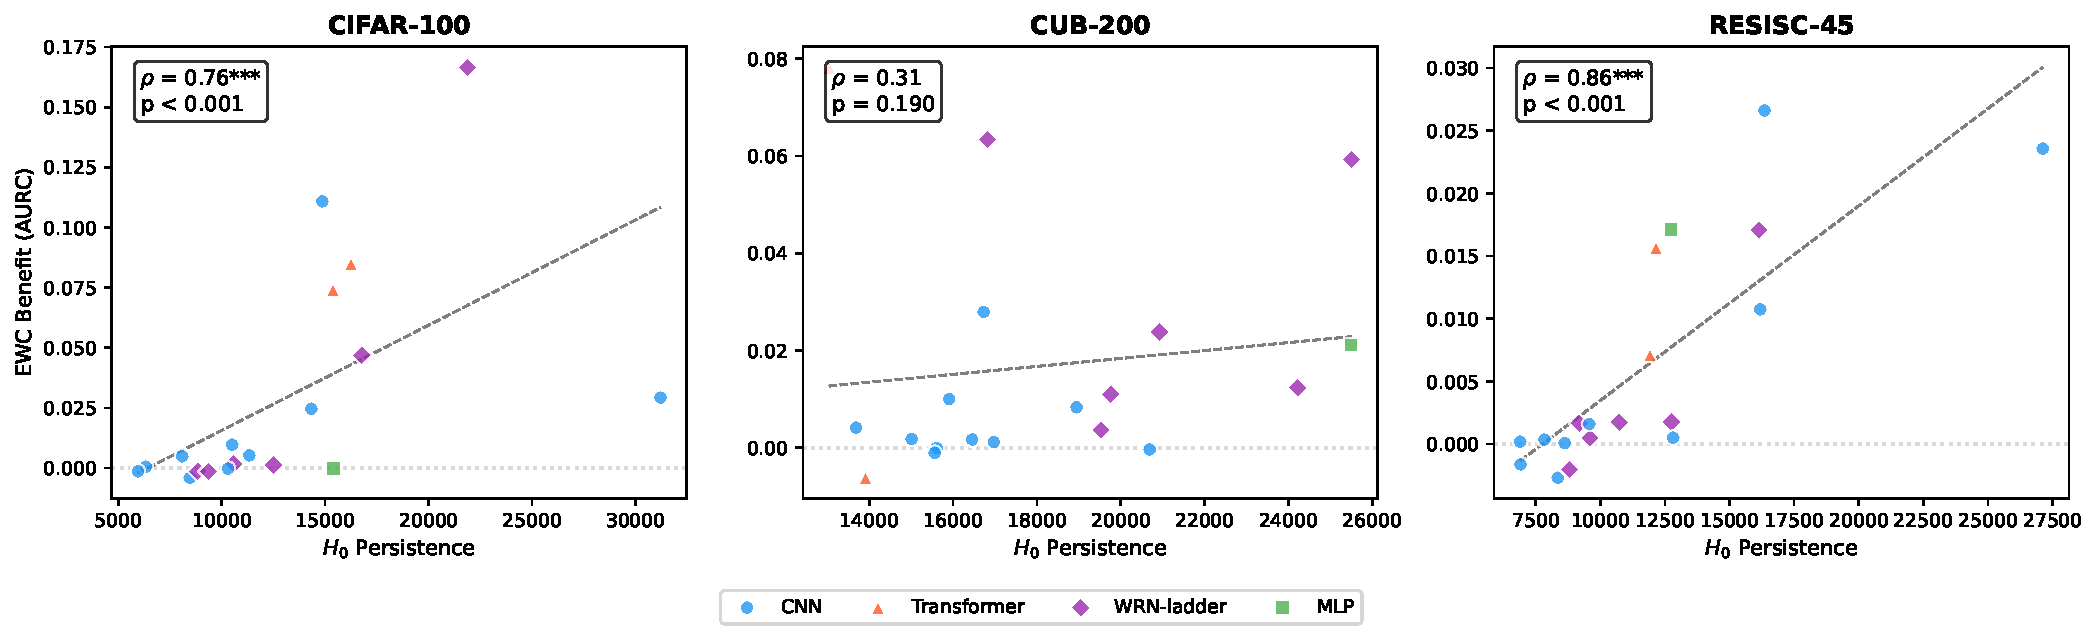
\includegraphics[width=\textwidth]{figures/h0_vs_ewc_benefit.pdf}
\caption{$H_0$ persistence vs.\ EWC benefit across 19 architectures per dataset. Strong positive correlation on CIFAR-100 ($\rho = 0.76$) and RESISC-45 ($\rho = 0.86$); null on CUB-200 ($\rho = 0.31$). Points colored by architecture family; dashed line is OLS fit. WRN-ladder points (purple diamonds) span the full H0 range within a single architecture family.}
\label{fig:h0_ewc_scatter}
\end{figure}

\begin{table}[t]
\centering
\caption{$H_0$ vs.\ EWC benefit. Spearman $\rho$ with bootstrap 95\% CI and Kendall $\tau$. Bold: survives Bonferroni ($\alpha = 0.004$).}
\label{tab:ewc_corr}
\small
\begin{tabular}{@{}lcccc@{}}
\toprule
Dataset & $\rho$ & 95\% CI & $p$ & $\tau$ \\
\midrule
CIFAR-100  & \textbf{0.76} & [0.46, 0.91] & \textbf{0.0002} & 0.57 \\
RESISC-45  & \textbf{0.86} & [0.65, 0.94] & $\mathbf{< 0.001}$ & 0.67 \\
CUB-200    & 0.31 & [$-$0.22, 0.78] & 0.190 & 0.26 \\
\bottomrule
\end{tabular}
\end{table}

\subsection{H0 Is Not Fully Reducible to Capacity}

Since $H_0$ correlates with model size (Section~\ref{sec:wrn}), the natural concern is that it merely proxies for parameter count. Table~\ref{tab:capacity_control} answers this directly. On RESISC-45, $H_0$ alone explains more variance ($R^2 = 0.645$) than parameter count ($R^2 = 0.242$), and remains highly significant in the joint model ($p < 0.001$). Pooled across datasets, $H_0$ retains significance ($p = 0.012$) with a partial correlation of $\rho = +0.33$ ($p = 0.013$). On CIFAR-100, $H_0$ is marginal ($p = 0.056$), directionally consistent but underpowered at $n = 19$; post-hoc power analysis indicates that $n = 19$ provides approximately 55\% power to detect an effect of this magnitude in a two-predictor model, suggesting the marginal result reflects limited sample size rather than absent signal. Adding depth as a third predictor does not reach significance on any dataset ($p > 0.26$) and does not change the $H_0$ coefficient.

\begin{table}[t]
\centering
\caption{Controlled regression: EWC benefit $\sim$ $\log(\text{params}) + H_0$. $H_0$ $p$ tests topology's contribution beyond model size. Bold: $p < 0.05$.}
\label{tab:capacity_control}
\small
\begin{tabular}{@{}lccccc@{}}
\toprule
Dataset & $R^2_{\text{params}}$ & $R^2_{H_0}$ & $R^2_{\text{both}}$ & $H_0$ $p$ & Partial $\rho$ \\
\midrule
CIFAR-100 ($n\!=\!19$)  & 0.527 & 0.304 & 0.626 & 0.056 & +0.39 \\
CUB-200 ($n\!=\!19$)    & 0.212 & 0.017 & 0.216 & 0.767 & +0.28 \\
RESISC-45 ($n\!=\!19$)  & 0.242 & 0.645 & \textbf{0.764} & $\mathbf{< 0.001}$ & \textbf{+0.63} \\
Pooled ($n\!=\!57$)      & 0.262 & 0.150 & 0.344 & \textbf{0.012} & \textbf{+0.33} \\
\bottomrule
\end{tabular}
\end{table}

\subsection{H0 Is Not Redundant with Cheaper Baselines}
\label{sec:baselines}

A stronger version of the proxy concern asks whether $H_0$ merely recapitulates information available from cheaper metrics. We test five baselines: Hessian trace (sharpness), maximum Hessian eigenvalue, Fisher information trace, normalized loss barrier (all computed alongside persistent homology), and L2 weight norm (computed from saved checkpoints; a near-zero-cost scalar). Table~\ref{tab:baselines} reports partial Spearman correlations between $H_0$ and EWC benefit after controlling for each baseline individually.

\begin{table}[t]
\centering
\caption{Partial Spearman $\rho$ of $H_0$ with EWC benefit after controlling for each baseline metric. Bold: $p < 0.05$. $H_0$ retains significance on CIFAR-100 and RESISC-45 regardless of which baseline is controlled, including the trivial L2 weight norm. No baseline retains significance after controlling for $H_0$ except weight norm and Fisher trace on RESISC-45.}
\label{tab:baselines}
\small
\begin{tabular}{@{}llcccc@{}}
\toprule
& & \multicolumn{2}{c}{$H_0$ partial (ctrl baseline)} & \multicolumn{2}{c}{Baseline partial (ctrl $H_0$)} \\
\cmidrule(lr){3-4} \cmidrule(lr){5-6}
Dataset & Baseline & $\rho$ & $p$ & $\rho$ & $p$ \\
\midrule
\multirow{5}{*}{CIFAR-100}
  & Hessian trace  & \textbf{0.72} & \textbf{0.002} & 0.19 & 0.471 \\
  & Max eigenvalue & \textbf{0.71} & \textbf{0.002} & 0.12 & 0.664 \\
  & Fisher trace   & \textbf{0.69} & \textbf{0.001} & $-$0.13 & 0.596 \\
  & Barrier (norm) & \textbf{0.57} & \textbf{0.011} & 0.24 & 0.314 \\
  & Weight norm    & \textbf{0.61} & \textbf{0.005} & 0.05 & 0.853 \\
\midrule
\multirow{5}{*}{RESISC-45}
  & Hessian trace  & \textbf{0.87} & $\mathbf{< 0.001}$ & $-$0.39 & 0.137 \\
  & Max eigenvalue & \textbf{0.85} & $\mathbf{< 0.001}$ & $-$0.20 & 0.451 \\
  & Fisher trace   & \textbf{0.81} & $\mathbf{< 0.001}$ & \textbf{$-$0.55} & \textbf{0.015} \\
  & Barrier (norm) & \textbf{0.71} & $\mathbf{< 0.001}$ & $-$0.02 & 0.943 \\
  & Weight norm    & \textbf{0.81} & $\mathbf{< 0.001}$ & \textbf{0.47} & \textbf{0.040} \\
\midrule
\multirow{3}{*}{CUB-200}
  & Hessian trace  & \textbf{0.56} & \textbf{0.025} & $-$0.25 & 0.356 \\
  & Max eigenvalue & \textbf{0.59} & \textbf{0.015} & 0.02 & 0.931 \\
  & Weight norm    & 0.27 & 0.270 & $-$0.10 & 0.684 \\
\bottomrule
\end{tabular}
\end{table}

On CIFAR-100 and RESISC-45, $H_0$ remains significant after controlling for every baseline ($p \leq 0.011$), including the trivially computed L2 weight norm ($p = 0.005$ and $p < 0.001$). The pattern is largely asymmetric: most baselines do not retain significance after controlling for $H_0$ (all $p > 0.13$ on CIFAR-100). On RESISC-45, Fisher trace ($p = 0.015$) and weight norm ($p = 0.040$) retain marginal partial signal after controlling for $H_0$, suggesting these metrics capture some independent information on this dataset, though $H_0$ remains the dominant predictor.

On CUB-200, where $H_0$ shows no raw correlation with EWC benefit ($\rho = 0.33$, $p = 0.17$), controlling for Hessian trace or max eigenvalue reveals a suppressed $H_0$ signal ($p = 0.025$ and $0.015$), suggesting these baselines act as confounders on this dataset. Weight norm shows no signal on CUB-200 in either direction.

This analysis addresses the concern that persistent homology is an expensive recapitulation of cheaper metrics. On the two datasets where the topology--benefit relationship is strongest, $H_0$ captures predictive signal beyond what sharpness, Fisher information, loss barriers, and weight norm provide.

\subsection{WRN Width Ladder: Topology Tracks Capacity}
\label{sec:wrn}

The WRN-28-$k$ width ladder ($k = 1, 2, 4, 6, 8, 10$) provides a controlled test within a single architecture family (Figure~\ref{fig:wrn_ladder}). $H_0$ persistence monotonically decreases with width ($\rho = -1.0$ vs.\ parameter count) on all 3 datasets, consistent with wider networks having smoother, less fragmented landscapes. The perfect monotonicity reflects the discrete width increments in the WRN ladder ($k = 1, 2, 4, 6, 8, 10$) rather than continuous measurement precision; with only 6 ordered points, monotonicity requires each successive width to maintain rank order, which is structurally expected given that wider networks have strictly more capacity. Cubical and Ripser $H_1$ show perfect rank agreement ($\rho = 1.0$), confirming that the topological measurement is method-independent.

\begin{figure}[t]
\centering
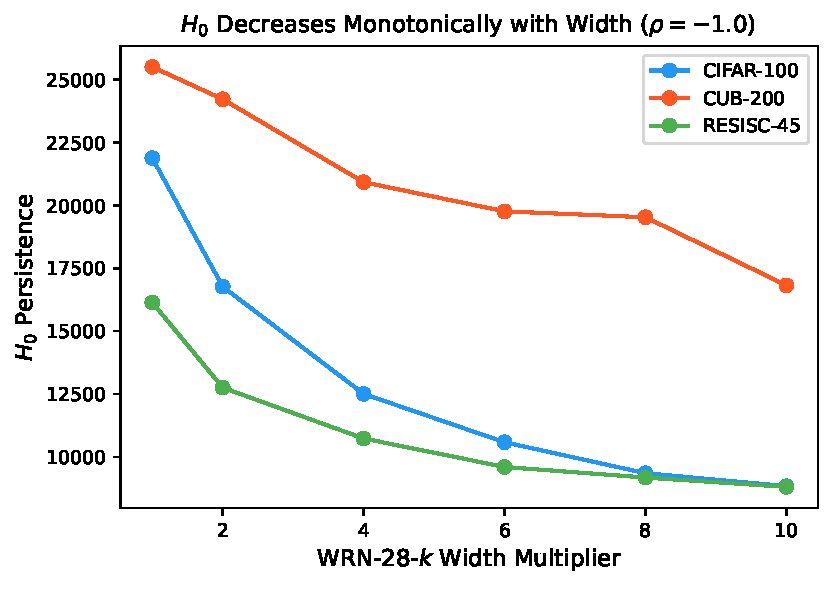
\includegraphics[width=0.6\textwidth]{figures/wrn_ladder_h0.pdf}
\caption{WRN-28-$k$ width ladder: $H_0$ decreases monotonically with width ($\rho = -1.0$) on all 3 datasets, consistent with wider networks having smoother, less fragmented landscapes.}
\label{fig:wrn_ladder}
\end{figure}

The width ladder demonstrates that the topology--capacity link is consistent across domains. It is the \emph{relationship between topology and mitigation benefit} that varies by task (Section~\ref{sec:dataset_variation}), not the topology--capacity link itself.

\subsection{Dataset-Dependent Moderation}
\label{sec:dataset_variation}

\textbf{Per-dataset forgetting prediction.} Leave-one-architecture-out (LOAO) Ridge regression with permutation testing shows topology's predictive value for raw forgetting is conditional on dataset (Table~\ref{tab:loao}). Topology rescues forgetting prediction on CUB-200 (permutation $p = 0.037$, suggestive but not surviving Bonferroni) where parameter count alone produces negatively correlated predictions ($\rho = -0.92$). On CIFAR-100, parameter count dominates and topology adds nothing. On RESISC-45, neither predictor set works for raw forgetting.

\begin{table}[t]
\centering
\caption{Per-dataset LOAO forgetting prediction. $\rho$: Spearman correlation between predicted and observed retention. Perm.\ $p$: permutation test for topology improvement over params. Bold: $p < 0.05$ (does not survive Bonferroni).}
\label{tab:loao}
\small
\begin{tabular}{@{}llccc@{}}
\toprule
Dataset & Outcome & Params $\rho$ & +Topo $\rho$ & Perm.\ $p$ \\
\midrule
CIFAR-100  & ret@100 & 0.43  & 0.30  & 0.295 \\
CUB-200    & ret@10  & $-$0.92 & \textbf{0.34} & \textbf{0.037} \\
RESISC-45  & ret@100 & $-$0.32 & $-$0.33 & 0.566 \\
\bottomrule
\end{tabular}
\end{table}

The CUB-200 result is notable: parameters alone systematically predict high retention for architectures that forget most (negative $\rho$), while topology corrects this. The matched-dimensionality null control confirms the CUB-200 improvement exceeds the 95th percentile of random features with the same dimensionality.

\textbf{Pooled interaction model.} The full interaction model (Equations 4--5) quantifies the observed moderation pattern: adding $H_0$ and its dataset interactions improves $R^2$ from 0.502 to 0.587 (permutation $p = 0.046$). Table~\ref{tab:partial_effects} presents the per-dataset partial effects with 95\% clustered bootstrap confidence intervals. For EWC benefit, the $H_0$ effect excludes zero on CIFAR-100 and RESISC-45 but not CUB-200, consistent with the per-dataset correlations in Table~\ref{tab:ewc_corr}. Notably, the retention outcome (ret@10) shows a different pattern: only CUB-200 excludes zero, suggesting that topology's relationship to raw forgetting vs.\ mitigation benefit involves different mechanisms. Figure~\ref{fig:pooled_interaction} visualizes the moderation pattern.

\begin{table}[t]
\centering
\caption{Per-dataset partial effect of $\tilde{H}_0$ (z-scored within dataset) from the pooled interaction model, with 95\% clustered bootstrap CIs. Bold: CI excludes zero.}
\label{tab:partial_effects}
\small
\begin{tabular}{@{}llrl@{}}
\toprule
Outcome & Dataset & Effect & 95\% CI \\
\midrule
\multirow{3}{*}{Retention (ret@10)}
  & CIFAR-100  & $-$0.001 & [$-$0.486, +0.073] \\
  & CUB-200    & \textbf{$-$0.123} & \textbf{[$-$0.183, $-$0.046]} \\
  & RESISC-45  & $-$0.021 & [$-$0.264, +0.083] \\
\midrule
\multirow{3}{*}{EWC benefit (AURC)}
  & CIFAR-100  & \textbf{+0.016} & \textbf{[+0.005, +0.062]} \\
  & CUB-200    & +0.002 & [$-$0.008, +0.013] \\
  & RESISC-45  & \textbf{+0.007} & \textbf{[+0.004, +0.012]} \\
\bottomrule
\end{tabular}
\end{table}

\begin{figure}[t]
\centering
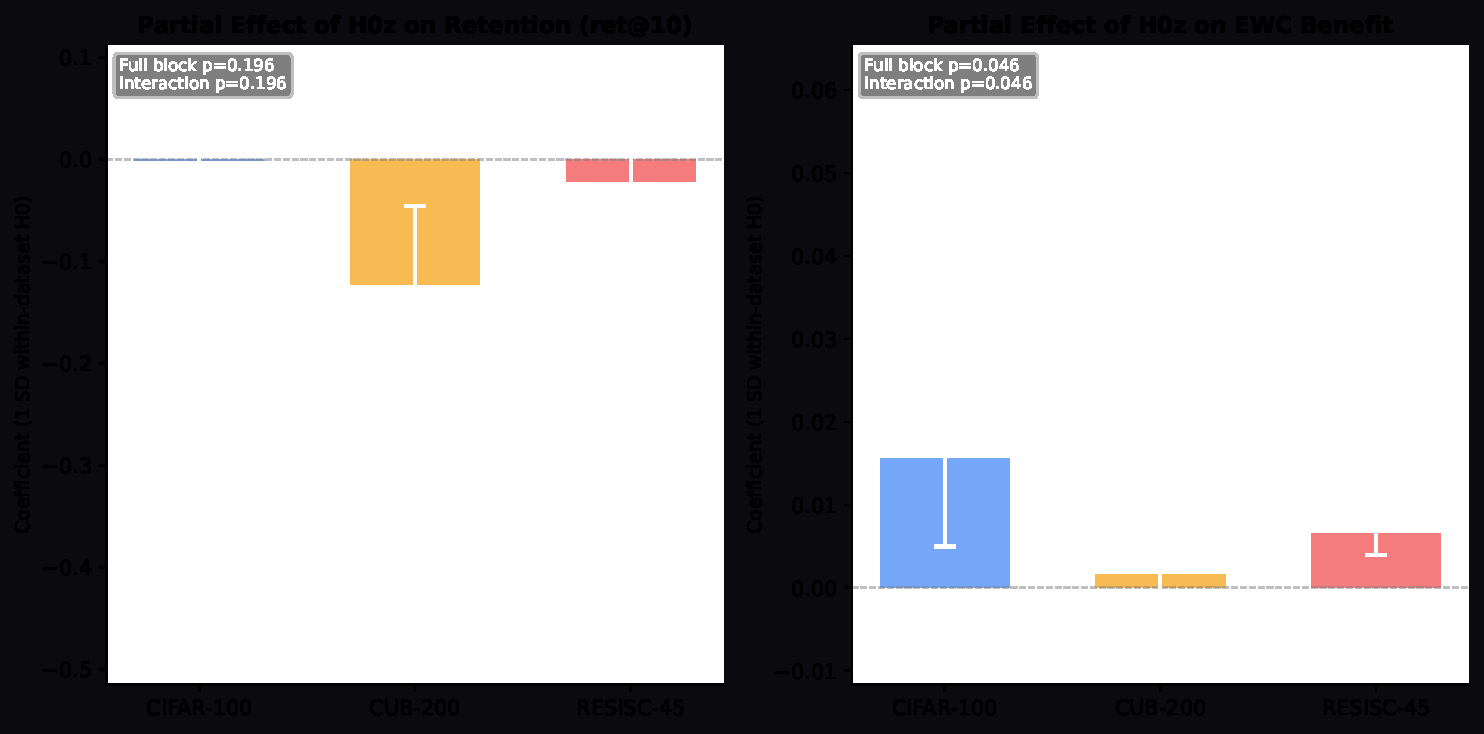
\includegraphics[width=\textwidth]{pooled_interaction_figure.pdf}
\caption{Per-dataset partial effects of within-dataset $\tilde{H}_0$ with 95\% clustered bootstrap CIs. Left: effect on retention (ret@10); only CUB-200 excludes zero. Right: effect on EWC benefit; CIFAR-100 and RESISC-45 exclude zero while CUB-200 does not, demonstrating dataset-dependent moderation (block permutation $p = 0.046$). The asymmetry between panels shows that topology relates to forgetting and mitigation benefit through different pathways.}
\label{fig:pooled_interaction}
\end{figure}

This result is exploratory (the model was designed after observing per-dataset patterns) and should be treated as hypothesis-generating. All VIF values fall below 3.5 in the z-scored specification.

\textbf{Influence diagnostics.} Cook's distance analysis identifies ConvNeXt-Tiny (CIFAR-100) as a high-leverage point ($D = 2.89$, threshold $4/n = 0.07$), driven by its unusual combination of high parameter count and high leverage in the design matrix. Five additional observations exceed the Cook's $D$ threshold. However, the maximum DFBETAS for the $\tilde{H}_0$ coefficient is 0.026, indicating that no single observation qualitatively alters the $H_0$ effect estimate. The presence of influential points in a 57-observation model underscores the need for replication with larger architecture samples.

\textbf{Robustness checks.} Three additional analyses support consistent inference: (i) a reduced model omitting $\hat{p} \times D$ interactions yields $p = 0.031$ for EWC benefit; (ii) using raw $H_0$ (not z-scored) produces the same qualitative conclusions; (iii) alternative outcome variables (ret@100) reach $p = 0.035$ in the pooled model, while the primary forgetting outcome (ret@10) does not reach significance ($p = 0.196$), consistent with the interpretation that topology relates more directly to mitigation benefit than to raw forgetting.

\subsection{Scale Validation: ImageNet-100}
\label{sec:scale}

The small-scale study establishes $H_0$ as the informative topological feature for models under 45M parameters trained from scratch. To test whether this extends to larger pretrained models, we evaluate 8 architectures (20M--304M parameters) fine-tuned on ImageNet-100 at $224 \times 224$ resolution (Table~\ref{tab:imagenet}).

\begin{table}[t]
\centering
\caption{ImageNet-100 Phase 4 correlations ($n = 8$). $H_1$, not $H_0$, is the dominant predictor at this scale. Bold: survives Bonferroni ($\alpha = 0.004$).}
\label{tab:imagenet}
\small
\begin{tabular}{@{}lcc@{}}
\toprule
Predictor & $\rho$ vs.\ retention & $p$ \\
\midrule
$H_1$ persistence & \textbf{0.93} & \textbf{0.0007} \\
Parameter count    & 0.52 & 0.183 \\
$H_0$ persistence  & $-$0.40 & 0.320 \\
\bottomrule
\end{tabular}
\end{table}

The notable observation is that $H_1$ (loops), not $H_0$ (connected components), shows the strongest correlation with retention at ImageNet-100 scale ($\rho = 0.93$, $p = 0.0007$, Bonferroni-significant at $p_{\text{bonf}} = 0.008$). $H_0$ is not significant ($\rho = -0.40$, $p = 0.32$), and parameter count alone does not predict retention ($\rho = 0.52$, $p = 0.18$). One hypothesis is that at larger scale with pretrained representations, the relevant landscape structure shifts from basin multiplicity ($H_0$) to basin connectivity ($H_1$). However, with $n = 8$ and a different training regime, this observation is preliminary and should not be interpreted as an established pattern.

\textbf{Four-dataset pooling ($n = 65$).} Adding ImageNet-100 to the pooled interaction model slightly dilutes the 3-dataset EWC benefit moderation (permutation $p$: $0.046 \to 0.063$). However, the reduced model (omitting $\hat{p} \times D$ interactions) retains significance ($p = 0.030$), and the original 3-dataset results replicate exactly when run independently. The dilution is expected: the small-scale $H_0$-based model is being pooled with a dataset where $H_1$, not $H_0$, carries the signal.

\textbf{Caveats.} The ImageNet-100 results have important limitations: (i) $n = 8$ provides low statistical power, and LOAO prediction does not reach significance (permutation $p = 0.978$); (ii) the experimental regime differs (pretrained fine-tuning vs.\ from-scratch training), so the dimension shift could reflect the pretrained landscape structure rather than a pure scale effect; (iii) the $H_1$ finding requires replication before strong claims are warranted.

\subsection{Method Specificity: SI Shows No Topology Moderation}
\label{sec:si}

This result is among the most informative in the study. SI \citep{zenke2017continual} is a second curvature-aware regularization method that uses online path integrals of per-parameter contributions rather than the post-hoc Fisher information matrix used by EWC. If the basin fragmentation hypothesis described a general property of curvature-based regularization, SI should show comparable topology moderation. It does not.

On ImageNet-100, we compute SI benefit alongside EWC benefit for all 8 architectures. The 4-dataset pooled interaction model yields $p = 1.000$ for SI benefit (both full block and interaction terms), indicating zero topology moderation. This refines the hypothesis: the topology--benefit relationship appears specific to EWC's Fisher-based penalty, not a general consequence of curvature-aware regularization. The distinction matters because it narrows the mechanism. EWC penalizes deviation from the original minimum weighted by per-parameter Fisher information (local curvature at the optimum). SI accumulates importance along the optimization path. If basin fragmentation determines how much a fixed-point penalty helps, it need not determine how much a path-integral penalty helps. The SI null directly addresses falsification target~1 (Section~\ref{sec:hypothesis}) and suggests a narrower hypothesis, from ``topology predicts regularization benefit'' to ``topology predicts Fisher-based regularization benefit.''

% ════════════════════════════════════════
\section{The Basin Fragmentation Hypothesis}
\label{sec:hypothesis}

The capacity-controlled results motivate a mechanistic hypothesis linking landscape topology to mitigation sensitivity.

$H_0$ persistence in the sublevel-set filtration counts connected components and their relative depths. High $H_0$ corresponds to a \emph{fragmented} landscape with many disconnected low-loss basins separated by high-loss barriers. We propose:

\begin{quote}
\textbf{Basin Fragmentation Hypothesis.} $H_0$ measures landscape fragmentation that determines how much curvature-based regularization helps by preventing inter-basin drift during sequential training.
\end{quote}

\textbf{The mechanism.} When the landscape is fragmented (high $H_0$), naive sequential training on a new task can push parameters across basin boundaries, causing them to settle in a basin that encodes the new task at the expense of the old. EWC penalizes deviations from the original minimum in proportion to Fisher information, constraining the optimization trajectory to remain near the original basin. This constraint is maximally beneficial when there are many basins to drift between (high $H_0$) and minimally beneficial when the landscape is smooth with a single broad basin (low $H_0$).

\textbf{Supporting evidence:}
\begin{enumerate}[nosep,leftmargin=*]
    \item $H_0$ predicts EWC benefit on CIFAR-100 ($\rho = 0.76$) and RESISC-45 ($\rho = 0.86$), surviving capacity controls on RESISC-45 ($p < 0.001$) and pooled ($p = 0.012$).
    \item The WRN width ladder shows $H_0$ monotonically decreases with width ($\rho = -1.0$), consistent with wider networks having less fragmented landscapes.
    \item CUB-200 shows no $H_0$--benefit relationship ($\rho = 0.31$, $p = 0.19$), consistent with a domain where forgetting mechanisms differ (see below).
    \item Preliminary evidence at larger scale ($n = 8$, ImageNet-100) suggests $H_1$ (loops) may carry the topological signal ($\rho = 0.93$), raising the possibility that the informative topological dimension shifts with scale. This observation requires replication before incorporation into the hypothesis.
\end{enumerate}

\textbf{CUB-200 as boundary condition.} The CUB-200 null ($\rho = 0.31$, $p = 0.19$) constitutes a boundary condition, not a failure to explain away. The mechanism behind CUB-200's divergence is uncertain: fine-grained discrimination may involve representational interference that is orthogonal to basin-level fragmentation, but we have not tested this. The partial effects (Table~\ref{tab:partial_effects}) show an intriguing asymmetry: topology relates to raw forgetting on CUB-200 (ret@10 CI excludes zero) but not EWC benefit, while the reverse holds for CIFAR-100 and RESISC-45. We present this as a pattern requiring investigation, not as evidence for a second mechanism.

\textbf{Implications for method selection.} If confirmed, the basin fragmentation hypothesis would provide directional signal for method selection: high-$H_0$ models may benefit more from Fisher-based regularization (EWC); low-$H_0$ models or fine-grained tasks might respond better to replay or architectural methods. The SI null (Section~\ref{sec:si}) is critical here: it narrows the scope from all curvature-aware methods to Fisher-based regularization specifically, suggesting that EWC's fixed-point penalty interacts with basin structure in a way that SI's path-integral penalty does not. This specificity is valuable because it constrains the mechanism rather than leaving it open to trivial explanations.

\textbf{Falsification targets and status.}
\begin{enumerate}[nosep,leftmargin=*]
    \item SI benefit shows no $H_0$ correlation (finding is EWC-specific). \textbf{Tested:} Confirmed. SI moderation $p = 1.000$ on ImageNet-100 (Section~\ref{sec:si}).
    \item Expanding to 50+ architectures eliminates the signal (small-sample artifact). \textit{Open.}
    \item SAM changes $H_0$ without changing EWC benefit (link is spurious). \textit{Open.}
    \item Cubical persistence disagrees with Ripser on the moderation result. \textbf{Not observed:} $H_1$ agreement $\rho = 1.0$ across all datasets.
    \item Replay-based methods show equal $H_0$ correlation (no curvature specificity). \textit{Open.}
\end{enumerate}

% ════════════════════════════════════════
\section{Limitations and Future Work}
\label{sec:limitations}

\textbf{Scale.} The small-scale study covers 19 architectures under 45M parameters. The ImageNet-100 scale validation extends to 304M parameters but with only $n = 8$ architectures in a different experimental regime (pretrained fine-tuning). Whether the $H_1$ signal at scale is robust requires replication with more architectures, and production-scale models (1B+) remain untested.

\textbf{Two-task sequences.} We test a single Task A $\rightarrow$ Task B transition. Real continual learning involves 10--100+ sequential tasks. Whether topology measured once remains predictive over long curricula is unexplored.

\textbf{Method specificity.} We test EWC and SI. The SI null narrows the hypothesis to EWC-specific effects. Replay-based and architecture-based methods have not been tested. The basin fragmentation hypothesis predicts that replay should show no $H_0$ correlation, but this remains unverified.

\textbf{Statistical power.} Per-dataset analyses operate on $n = 19$ (small-scale) or $n = 8$ (ImageNet-100). The CIFAR-100 controlled regression is marginal ($p = 0.056$). The pooled interaction model ($p = 0.046$) was designed after observing per-dataset patterns and does not survive strict correction.

\textbf{2D slice fidelity.} The signal depends on 2D cross-sections of a high-dimensional surface. Five slices reduce sampling variance but do not guarantee that $H_0$ or $H_1$ in 2D faithfully approximates true basin structure.

\textbf{Exploratory design.} The EWC benefit analysis was not part of the original study plan (Section~\ref{sec:transparency}). The controlled regression was conducted after observing bivariate correlations. These results require pre-registered confirmatory replication.

\textbf{Future work.} Immediate priorities: (i) replicate the $H_1$ finding at scale with 20+ pretrained architectures; (ii) test PackNet and experience replay to evaluate method generalization beyond EWC/SI; (iii) pre-register the capacity-controlled regression on expanded architecture samples (50+). Additional directions: testing whether topological diagnostics add value beyond simpler baselines (e.g., weight norm) in other learning dynamics such as grokking \citep{power2022grokking}; extending to NLP tasks, long task sequences, and causal interventions (manipulating fragmentation via SAM).

% ════════════════════════════════════════
\section{Analysis Path Transparency}
\label{sec:transparency}

The original study targeted topology as a direct forgetting predictor. CIFAR-100 ran first, revealing parameter count dominance. CUB-200 showed topology rescues prediction where parameters fail. RESISC-45 produced a null. The EWC benefit finding emerged from diagnostic analysis and was not pre-specified. The pooled interaction model was designed after observing per-dataset EWC patterns. The controlled regression (Table~\ref{tab:capacity_control}) was conducted after observing that $H_0$ and parameter count are correlated. The ImageNet-100 scale validation and SI testing were planned after the 3-dataset results were complete, motivated by the falsification targets. We report these as discoveries requiring confirmation, not as confirmatory evidence.

% ════════════════════════════════════════
\section{Conclusion}
\label{sec:conclusion}

We introduce a geometric lens on mitigation sensitivity in continual learning. Across 27 architectures and 4 datasets (65 configurations), we show that $H_0$ persistent homology of loss landscapes provides predictive signal for the magnitude of EWC benefit under specific dataset conditions, and that this signal survives after controlling for model capacity. The effect is strongest on RESISC-45 ($R^2 = 0.645$ vs.\ $0.242$ for parameter count, $p < 0.001$), replicates on CIFAR-100, and is absent on CUB-200. Pooled across the 3 small-scale datasets ($n = 57$), $H_0$ retains significance ($p = 0.012$) after capacity and depth controls.

Preliminary scale validation on ImageNet-100 ($n = 8$) suggests $H_1$ (loops) may replace $H_0$ as the informative topological feature at larger scale ($\rho = 0.93$, $p = 0.0007$), though the different training regime and small sample limit this observation. The SI null ($p = 1.000$) is among the study's most informative results: it sharpens the hypothesis from general curvature-based regularization to EWC-specific Fisher-based regularization, narrowing the mechanism and providing preliminary evidence against a trivially general interpretation.

While topology explains variance in EWC benefit beyond all tested baselines, its out-of-sample predictive performance (LOAO) is dataset-dependent and not uniformly improved over parameter-based models. The strength of the current evidence is in variance explanation and controlled regression, not in consistent cross-architecture prediction.

The basin fragmentation hypothesis offers a testable mechanism with explicit falsification targets, one of which (SI specificity) has already been confirmed. These results are preliminary: the effect appears on two of three small-scale datasets (strongest on RESISC-45, replicated on CIFAR-100), CUB-200 constitutes an unexplained boundary condition, and the scale validation has only $n = 8$. Whether the geometric lens holds robustly at production scale remains the central open question. We view this work as hypothesis-generating empirical science aimed at identifying structure that future theory should explain, and commit to pre-registered confirmatory replication.

% ════════════════════════════════════════
\bibliography{../references}
\bibliographystyle{collas2026_conference}

\end{document}
